\documentclass[10pt,twocolumn]{article}
\usepackage[a4paper,margin=15mm]{geometry}
\usepackage{amsmath,amssymb}
\usepackage{amsthm}
\usepackage{graphicx}
\theoremstyle{plain}
\newtheorem{theorem}{Theorem}
\newtheorem{proposition}[theorem]{Proposition}
\newtheorem{corollary}[theorem]{Corollary}
\theoremstyle{definition}
\newtheorem{definition}[theorem]{Definition}
\theoremstyle{remark}
\newtheorem{remark}[theorem]{Remark}
\usepackage{booktabs,array,calc}
\usepackage[font=small,labelfont=bf]{caption}
\usepackage[colorlinks=true]{hyperref}
\usepackage{etoolbox}
\providecommand{\tightlist}{\setlength{\itemsep}{0pt}\setlength{\parskip}{0pt}}
\renewcommand{\thesubsection}{\arabic{subsection}.}
\emergencystretch=3em
\allowdisplaybreaks
\setlength{\tabcolsep}{3.6pt}
\AtBeginDocument{%
  \BeforeBeginEnvironment{equation}{\small}%
  \BeforeBeginEnvironment{equation*}{\small}%
  \BeforeBeginEnvironment{align}{\small}%
  \BeforeBeginEnvironment{align*}{\small}%
  \BeforeBeginEnvironment{gather}{\small}%
  \BeforeBeginEnvironment{gather*}{\small}%
}

\begin{document}
\title{Probabilistic Sufficiency for the Obstruction Calculus:\\
Belief-State Safety Values under Partial Observation}
\author{Amin Abaee\\[0.35em]
{\small Independent Researcher}\\[0.55em]
{\small\href{https://orcid.org/0000-0002-0019-1842}{ORCID: 0000-0002-0019-1842}}\\[0.3em]
{\small\href{mailto:amin\_abaee@ut.ac.ir}{amin\_abaee@ut.ac.ir}}}
\date{September 26, 2026}
\maketitle

\begin{abstract}
The obstruction calculus characterizes nonviability through certificates on
information states; the probabilistic side asks what the certificates imply
when the information state is a distribution. This paper consolidates the
probabilistic programme into one standalone development of the belief-state
safety value \(V_{k}(b)\) --- the maximal probability of remaining safe for
\(k\) steps under the disturbance's worst case --- and establishes four
results. First, a support identity: on finite models with deterministic
kernels the posterior support coincides with the set-valued post-state of
the calculus, the value-one level of the recursion coincides with the
viable-set recursion \(\mathcal{W}_{k}\), and outside it the deficit
satisfies \(1 - V_{k}(b) \ge \min_{x \in \mathrm{supp}(b)} b(x)\), attained
on natural instances. Second, exactness: over rational input data the
finite-horizon values are piecewise linear with rational alpha-vectors, so
all values are exact rationals computable without floating point; the
verification campaign's 384 vectors are all exact, realizing exactly three
types (\(156\), \(156\), and \(72\) occurrences), and the complete
\(16 \times 12\) value table over the audited grid is carried here. Third,
agreement on the audited delayed-regime class: a class-restricted
alpha-vector recursion reproduces the closed-form values on all 48 audited
cells and horizons \(k \le 4\), the certificate partition coincides with
the value boundaries, and the value jumps by exactly \(1/2\) at
\(z_{0} = 1 + \min(k, T_{\mathrm{obs}})\); the declared hold class equals
the unrestricted sequential blind class at the one-step horizon, and for
horizons \(k \ge 2\) the two differ exactly on the timing cells
(\(2 \le z_{0} < 1 + T_{\mathrm{obs}}\)), where open-loop time-variation
within the blind window lifts the value to one --- 36 cell-horizon
combinations in all, enumerated in full. Fourth, adaptive observation: on
the declining hidden-parameter instance a single probe reveals the
parameter exactly (branch separation \(2\)), survival forces
\(z_{0} \ge 21/10\), and under revelation at horizon
\(T_{\mathrm{learn}}\) viability holds exactly when
\(z_{0} \ge 21/10 + T_{\mathrm{learn}}/10\) --- the learning deadline acts
as the timing obstruction's observation deadline, and the kernel shrinks
linearly and antitone in it (\(|K| = 5, 4, 3, 2, 1\)). All computations run
in exact rational arithmetic; the complete audited tables, the derivations
behind the closed form and the class declaration, and the five-figure set
are regenerated by the chained verification scripts.
\end{abstract}

\textbf{Keywords:} partially observable control; viability kernels;
belief states; safety values; exact arithmetic; adaptive observation

\subsection{Introduction}\label{introduction}

Viability under incomplete observation divides into a necessity side and a
sufficiency side. The obstruction calculus treats the necessity side:
certificates whose firing proves nonviability of an information state
(Abaee, 2026b). The probabilistic question is the quantitative counterpart.
If the controller holds a distribution \(b\) over states rather than a set,
how safe is safe? The answer is a function: the belief-state safety value
\(V_{k}(b)\), the maximal worst-case probability of keeping the state
trajectory in the safe set for \(k\) steps. Its value-one level is the
viability statement of the set-valued theory; everything below level one
is measured by the deficit \(1 - V_{k}(b)\), and the obstruction
certificates reappear as lower bounds on that deficit.

This paper is the probabilistic-sufficiency flagship of the calculus
programme: it consolidates the stochastic selector development, the
belief-state value campaign, and the hidden-parameter learning-deadline
audit into one standalone theory, per the programme's consolidation
decision. The companion papers are unchanged by it: the calculus paper
records the set-valued theory and previews this development in its
probabilistic section; the computational companion certifies the finite
programmes and packages the exact recursion as a reference library; the
worked-systems companion audits the catalogue's count identities. Nothing
verified in the companions is re-proved differently here; this paper
carries the probabilistic layer they delimit.

The development proceeds in seven steps. Section \ref{model} states the
augmented model --- total transition rows, an absorbing unsafe state
carrying its own observation, masked witnesses --- and the value recursion,
distinguishing the selector's attaining set from its value-one level.
Section \ref{support} connects the belief-state recursion to the
set-valued recursion of the calculus exactly, through the support of the
belief. Section \ref{exact} shows the finite-horizon values are piecewise
linear and exactly representable, and carries the complete audited value
table over the delayed grid. Section \ref{deterministic} evaluates the
deterministic limit, at which the recursion degenerates to a
survived-mass formula over blind action sequences, with the asymmetric
audit carried sequence by sequence. Section \ref{deficit} reads the
obstruction certificates systematically as deficit lower bounds. Section
\ref{agreement} proves agreement between the class-restricted value
recursion and the closed-form values on the audited delayed-regime class,
quantifies what the class declaration contributes, locates the value's
jump loci, and carries the derivations. Section \ref{adaptive} treats
observation as a design variable: probes, learning deadlines, and the
exact kernel cost of late resolution of a hidden parameter.

All audited computations are exact: integer and rational arithmetic,
standard library only, deterministic scripts (Section \ref{methods}).

\subsection{The augmented model, the safety value, and the selector}\label{model}

\emph{The augmented state space.} Let the physical safe set be
\(\mathcal{V}\) and let the state space of the model be
\(X^{\perp} = \mathcal{V} \cup \{\bot\}\), where \(\bot\) is an absorbing
unsafe state. For \(x \in \mathcal{V}\) the transition row splits between
\(\mathcal{V}\) and \(\bot\),
\[
\textstyle\sum_{x' \in \mathcal{V}} T(x' \mid x, a) \le 1,\quad
T(\bot \mid x, a) = 1 - \sum_{x' \in \mathcal{V}} T(x' \mid x, a),
\]
and the bottom row is \(T(\bot \mid \bot, a) = 1\): every row of \(T\)
sums to one and \(\bot\) is absorbing, so exit from \(\mathcal{V}\) is
absorption and no trajectory re-enters \(\mathcal{V}\) from outside it.
The observation model is completed on all of \(X^{\perp}\): there is a
distinguished observation \(y_{\bot}\) with
\(g(y_{\bot} \mid \bot, a, \bot) = 1\) (and
\(g(y \mid \cdot, \cdot, \bot) = 0\) for \(y \ne y_{\bot}\)), while
\(g(\cdot \mid x, a, x')\) on \(\mathcal{V}\) is arbitrary non-negative
with the usual normalization per \((x, a)\). A belief is a distribution
\(b\) over \(X^{\perp}\), updated by Bayes' rule \(\tau(b, a, y)\), with
\(\mathbb{P}(y \mid b, a) = \sum_{x, x'} b(x)\, T(x' \mid x, a)\,
g(y \mid x, a, x')\); because every row sums to one and every
\((x, a, x')\) emits exactly one observation with probability one, the
laws \(\mathbb{P}(y \mid b, a)\) sum to one over \(y\) at every belief ---
no sub-probability bookkeeping is needed. On the deterministic kernels of
the audited instances this formalism converts set-valued nonviability into
almost-sure nonviability on the augmented chain.

\begin{definition}[safety value]\label{def:value}
Fix a declared policy class \(\Pi\). The safety value at horizon \(k\) is
the maximal class-survival probability
\[
V^{\Pi}_{k}(b) = \max_{\pi \in \Pi}\; \mathbb{P}_{\pi}\bigl( x_{t} \in
\mathcal{V} \text{ for } t = 0, \dots, k \;\big|\; b \bigr),
\]
the horizon counting the current state. The unrestricted class
\(\Pi = \Pi_{\mathrm{seq}}\) is the class of all sequential policies.
\end{definition}

\emph{The selector and its levels.} In the selector framework this is the
distributional counterpart of the recursive correspondence: the
information state is \(b\), a response is a class-admissible policy
segment. Two objects must be distinguished. The \emph{attaining set} at
\(b\),
\[
\Gamma^{\mathrm{s}}_{k}(b) = \Bigl\{ a \in A : \textstyle\sum_{y}
\mathbb{P}(y \mid b, a)\, V^{\Pi}_{k-1}\bigl(\tau(b, a, y)\bigr)
= V^{\Pi}_{k}(b) \Bigr\},
\]
collects the actions attaining the value; for finite \(A\) it is nonempty
at every belief and horizon --- nonemptiness is automatic and carries no
viability content. The \emph{value-one level},
\[
S^{\Pi}_{k}(b) = \Bigl\{ a \in A : \textstyle\sum_{y} \mathbb{P}(y \mid
b, a)\, V^{\Pi}_{k-1}\bigl(\tau(b, a, y)\bigr) = 1 \Bigr\},
\]
is the selector's viable-response set, and its nonemptiness corresponds
exactly to \(V^{\Pi}_{k}(b) = 1\). Obstruction certificates correspond to
deficits \(1 - V^{\Pi}_{k}(b) > 0\).

\begin{theorem}[belief-state value recursion]\label{thm:recursion}
\(V^{\Pi}_{0}(b) = b(\mathcal{V})\) (the horizon counts the current
state), and for \(k \ge 0\),
\[
V^{\Pi}_{k+1}(b) = \max_{a \in A(\Pi)}\; \sum_{y \in Y} \mathbb{P}(y \mid
b, a)\; V^{\Pi}_{k}\bigl(\tau(b, a, y)\bigr),
\]
where \(A(\Pi)\) is the class-admissible action set at the current stage
for Markov classes \(\Pi\). The recursion is exact on every finite
horizon; over the unrestricted class it is the Smallwood--Sondik
belief-state value iteration specialized to the absorbing safety reward
(Smallwood and Sondik, 1973).
\end{theorem}

The proof is standard value iteration for the belief-state Markov decision
process, with the absorbing state making \(V^{\Pi}_{k}\) the \(k\)-step
class-survival probability (Bertsekas and Shreve, 1978). For non-Markov
classes (the hold and open-loop classes of Section \ref{agreement}) the
class constraint couples stages; the audited computations there use the
equivalent segment form of Proposition \ref{prop:pl} below.

\subsection{The support identity and exact sufficiency}\label{support}

The bridge to the set-valued theory runs through the support. Write
\(\mathrm{supp}(b)\) for the states carrying positive mass, and let
\(\mathcal{W}_{k}\) denote the calculus's viable-set recursion:
\(\mathcal{W}_{0} = \{B \subseteq \mathcal{V}\}\) and
\(\mathcal{W}_{k} = \{B : \text{some admissible } a \text{ maps every }
x \in B \text{ into } \mathcal{W}_{k-1}\text{-supported posteriors}\}\).

\begin{theorem}[support identity]\label{thm:support}
On finite models with deterministic kernels, for every action \(a\) and
observation \(y\),
\[
\mathrm{supp}\bigl(b^{+}(\cdot \mid a, y)\bigr)
\;=\; \mathrm{Post}\bigl(\mathrm{supp}(b), a, y\bigr),
\]
the set-valued post-state of the calculus. Consequently
\(V_{k}(b) = 1\) if and only if
\(\mathrm{supp}(b) \in \mathcal{W}_{k}\), while if
\(\mathrm{supp}(b) \notin \mathcal{W}_{k}\) then every action loses a
compatible state of positive mass, so
\[
1 - V_{k}(b) \;\ge\; \min_{x \in \mathrm{supp}(b)} b(x).
\]
Moreover \(V_{k}(b)\) is non-increasing in \(k\).
\end{theorem}

\begin{corollary}[closed form on the delayed class]\label{cor:closed}
On the delayed hidden-regime instance --- states \((z, \theta)\) with
\(\theta \in \{-1, +1\}\), prior \(b_{0} = (\tfrac{1}{2}, \tfrac{1}{2})\)
from \(z_{0}\), no observation before \(T_{\mathrm{obs}}\), exact
revelation at \(T_{\mathrm{obs}}\), blind-window holds
\(u \equiv \pm 1\), and unit drift against the floors --- the belief
support follows the two branches \(z_{0} \mp k\), and
\[
\small
V_{k}(b_{0}) \;=\;
\begin{cases}
\tfrac{1}{2}\,\bigl(\mathbb{1}[z_{0} - k \ge 1] + \mathbb{1}[z_{0} + k \ge 1]\bigr), & k \le T_{\mathrm{obs}},\\[1ex]
\tfrac{1}{2}\,\bigl(1 + \mathbb{1}[z_{0} \ge 1 + T_{\mathrm{obs}}]\bigr), & k > T_{\mathrm{obs}}.
\end{cases}
\]
In particular \(V_{k}(b_{0}) = 1\) exactly on the viable region
\(z_{0} \ge 1 + T_{\mathrm{obs}}\), recovering the deterministic verdict
as the value-one level.
\end{corollary}

\begin{proof}[Derivation of Corollary \ref{cor:closed}]
While \(k \le T_{\mathrm{obs}}\) no observation arrives, so a policy
commits to one blind hold \(u \equiv \pm1\): under \(u \equiv +1\) the
\(\theta = +1\) branch sits at \(z_{0} + k\) at the horizon and the
\(\theta = -1\) branch at \(z_{0} - k\); under \(u \equiv -1\) the roles
swap. Each branch carries mass \(\tfrac{1}{2}\) and survives exactly when
it stays at or above the floor, giving
\(\tfrac{1}{2}(\mathbb{1}[z_{0} - k \ge 1] + \mathbb{1}[z_{0} + k \ge 1])\),
and the adversary cannot do better than pick the falling branch because
the infimum over disturbance strategies selects the branch.
For \(k > T_{\mathrm{obs}}\), revelation at \(T_{\mathrm{obs}}\) splits
the belief: the learned law \(u = \theta\) regenerates the realized
branch, so survival reduces to surviving the blind window of length
\(T_{\mathrm{obs}}\) on both branches --- the mass-\(\tfrac12\) falling
branch sits at \(z_{0} - T_{\mathrm{obs}}\) at revelation, whence the
indicator \(\mathbb{1}[z_{0} \ge 1 + T_{\mathrm{obs}}]\) weighting the
certainly-saved mass \(\tfrac{1}{2}\).
\end{proof}

\subsection{Exact piecewise-linear values}\label{exact}

\begin{proposition}[rational alpha-vectors, class-restricted]\label{prop:pl}
Fix a declared class \(\Pi\). At every horizon \(k\),
\(V^{\Pi}_{k}\) is piecewise linear and convex:
\(V^{\Pi}_{k}(b) = \max_{\alpha \in \Gamma^{\Pi}_{k}} \alpha^{\top} b\)
for a finite witness set \(\Gamma^{\Pi}_{k}\) on
\(\mathbb{Q}^{|\mathcal{V}|+1}\) (coordinates indexed by
\(\mathcal{V} \cup \{\bot\}\)), constructed by the masked backup
\[
\alpha^{a,\,\gamma_{\cdot}}(x) =
\sum_{x'} T(x' \mid x, a) \sum_{y} g(y \mid x, a, x')\, \gamma_{y}(x'),\quad
\gamma_{y} \in \Gamma^{\Pi}_{k},
\]
with \(\Gamma^{\Pi}_{0} = \{ \mathbf{1}_{\mathcal{V}} \}\) and the
boundary condition \(\alpha(\bot) = 0\) applied at every backup (the
backup acts on \(\mathcal{V}\) only; the \(\bot\)-coordinate of every
witness is anchored at zero and remains zero under the backup) and
\(\Gamma^{\Pi}_{k+1} = \{ \alpha^{a, \gamma_{\cdot}} : a \in A(\Pi),\
\gamma_{\cdot} \text{ a selection} \}\), duplicates removed by exact
equality. For a blind open-loop window the equivalent segment form
applies: each admissible action segment \((u_{0}, \dots, u_{m}) \in \Pi\)
contributes the witness
\(\alpha^{\mathrm{seg}} = (\mathbf{1}[\text{the segment saves branch } x])_{x}\)
and \(V^{\Pi}_{k}(b) = \max_{\mathrm{seg}} \alpha^{\mathrm{seg}\top} b\).
Over rational \(T\), \(g\), and priors, every \(\alpha\) is an exact
rational vector, every \(V^{\Pi}_{k}(b)\) at a rational belief is an exact
rational, and the attaining witness is part of the computation. The
worst-case growth is
\(|\Gamma^{\Pi}_{k+1}| \le |A|\,|\Gamma^{\Pi}_{k}|^{|Y|}\);
deduplication and pruned selections are the practical controls, and the
exponential law is the honest complexity statement for the general class.
\end{proposition}

The PL structure is Smallwood--Sondik's; the masking factor anchors
\(\alpha(\bot) = 0\) (survival requires the current state in
\(\mathcal{V}\), and \(\bot\) is absorbing, so no backup can revive a lost
branch). The exact-arithmetic discipline is the point: the backup maps
rational vectors to rational vectors by finite sums and products,
selections are finite, and equality tests for deduplication are exact on
rationals. In the verification campaign the alpha-vectors of all audited
instances --- 384 vectors across the two-floor instance and the delayed
grid --- are exact rationals.

\begin{remark}[dimension]\label{rem:dim}
On the two-floor instance the value function on the one-dimensional
simplex is \(\max(b_{0}, b_{1})\) for all audited horizons (Figure
\ref{fig:twofloor}); the witness alpha-vectors live in the two-coordinate
display, with the suppressed bottom coordinate identically zero --- padded
to \((1,0,0), (0,1,0)\) on \(\mathcal{V} \cup \{\bot\}\).
\end{remark}

On the delayed grid the campaign evaluates
\(\alpha_{k}(z_{0}, T_{\mathrm{obs}})\) at all
\(16 \times 3 \times 4 = 192\) cell-horizon combinations of
\(z_{0} \in \{1.0, 1.1, \dots, 2.5\}\),
\(T_{\mathrm{obs}} \in \{1, 2, 3\}\), \(k \in \{1, 2, 3, 4\}\). The
realized vectors take exactly three types: \((1, 1)\) (both branches
savable in the blind window), \(72\) occurrences; and the mirror pair
\((1, 0)\) and \((0, 1)\) (one branch savable), \(156\) occurrences each
--- the symmetry between the two mirror types is exact,
\(72 + 156 + 156 = 384\). Table \ref{tab:campaign} carries the complete
value table; Figure \ref{fig:staircase} displays the closed forms.

\begin{table*}[t]
\centering
\footnotesize
\caption{The complete audited value table on the delayed grid: the exact
\(V_{k}(b_{0})\) (values \(1\) or \(\tfrac{1}{2}\)) for all 16 grid
states, three blind-window lengths, four horizons --- 192 cell-horizon
combinations, each regenerated by script and each equal to both the
alpha-vector recursion and the closed form of Corollary
\ref{cor:closed}.}
\label{tab:campaign}
\begin{tabular}{@{}l cccc c@{\hspace{9pt}}cccc c@{\hspace{9pt}}cccc@{}}
\toprule
 & \multicolumn{4}{c}{$T_{\mathrm{obs}} = 1$}
 & \multicolumn{4}{c}{$T_{\mathrm{obs}} = 2$}
 & \multicolumn{4}{c}{$T_{\mathrm{obs}} = 3$}\\
\cmidrule(lr){2-5}\cmidrule(lr){6-9}\cmidrule(lr){10-13}
$z_0$ & $k{=}1$ & $k{=}2$ & $k{=}3$ & $k{=}4$
 & $k{=}1$ & $k{=}2$ & $k{=}3$ & $k{=}4$
 & $k{=}1$ & $k{=}2$ & $k{=}3$ & $k{=}4$\\
\midrule
1.0 & $\tfrac12$ & $\tfrac12$ & $\tfrac12$ & $\tfrac12$ & $\tfrac12$ & $\tfrac12$ & $\tfrac12$ & $\tfrac12$ & $\tfrac12$ & $\tfrac12$ & $\tfrac12$ & $\tfrac12$\\
1.1 & $\tfrac12$ & $\tfrac12$ & $\tfrac12$ & $\tfrac12$ & $\tfrac12$ & $\tfrac12$ & $\tfrac12$ & $\tfrac12$ & $\tfrac12$ & $\tfrac12$ & $\tfrac12$ & $\tfrac12$\\
1.2 & $\tfrac12$ & $\tfrac12$ & $\tfrac12$ & $\tfrac12$ & $\tfrac12$ & $\tfrac12$ & $\tfrac12$ & $\tfrac12$ & $\tfrac12$ & $\tfrac12$ & $\tfrac12$ & $\tfrac12$\\
1.3 & $\tfrac12$ & $\tfrac12$ & $\tfrac12$ & $\tfrac12$ & $\tfrac12$ & $\tfrac12$ & $\tfrac12$ & $\tfrac12$ & $\tfrac12$ & $\tfrac12$ & $\tfrac12$ & $\tfrac12$\\
1.4 & $\tfrac12$ & $\tfrac12$ & $\tfrac12$ & $\tfrac12$ & $\tfrac12$ & $\tfrac12$ & $\tfrac12$ & $\tfrac12$ & $\tfrac12$ & $\tfrac12$ & $\tfrac12$ & $\tfrac12$\\
1.5 & $\tfrac12$ & $\tfrac12$ & $\tfrac12$ & $\tfrac12$ & $\tfrac12$ & $\tfrac12$ & $\tfrac12$ & $\tfrac12$ & $\tfrac12$ & $\tfrac12$ & $\tfrac12$ & $\tfrac12$\\
1.6 & $\tfrac12$ & $\tfrac12$ & $\tfrac12$ & $\tfrac12$ & $\tfrac12$ & $\tfrac12$ & $\tfrac12$ & $\tfrac12$ & $\tfrac12$ & $\tfrac12$ & $\tfrac12$ & $\tfrac12$\\
1.7 & $\tfrac12$ & $\tfrac12$ & $\tfrac12$ & $\tfrac12$ & $\tfrac12$ & $\tfrac12$ & $\tfrac12$ & $\tfrac12$ & $\tfrac12$ & $\tfrac12$ & $\tfrac12$ & $\tfrac12$\\
1.8 & $\tfrac12$ & $\tfrac12$ & $\tfrac12$ & $\tfrac12$ & $\tfrac12$ & $\tfrac12$ & $\tfrac12$ & $\tfrac12$ & $\tfrac12$ & $\tfrac12$ & $\tfrac12$ & $\tfrac12$\\
1.9 & $\tfrac12$ & $\tfrac12$ & $\tfrac12$ & $\tfrac12$ & $\tfrac12$ & $\tfrac12$ & $\tfrac12$ & $\tfrac12$ & $\tfrac12$ & $\tfrac12$ & $\tfrac12$ & $\tfrac12$\\
2.0 & $1$ & $1$ & $1$ & $1$ & $1$ & $\tfrac12$ & $\tfrac12$ & $\tfrac12$ & $1$ & $\tfrac12$ & $\tfrac12$ & $\tfrac12$\\
2.1 & $1$ & $1$ & $1$ & $1$ & $1$ & $\tfrac12$ & $\tfrac12$ & $\tfrac12$ & $1$ & $\tfrac12$ & $\tfrac12$ & $\tfrac12$\\
2.2 & $1$ & $1$ & $1$ & $1$ & $1$ & $\tfrac12$ & $\tfrac12$ & $\tfrac12$ & $1$ & $\tfrac12$ & $\tfrac12$ & $\tfrac12$\\
2.3 & $1$ & $1$ & $1$ & $1$ & $1$ & $\tfrac12$ & $\tfrac12$ & $\tfrac12$ & $1$ & $\tfrac12$ & $\tfrac12$ & $\tfrac12$\\
2.4 & $1$ & $1$ & $1$ & $1$ & $1$ & $\tfrac12$ & $\tfrac12$ & $\tfrac12$ & $1$ & $\tfrac12$ & $\tfrac12$ & $\tfrac12$\\
2.5 & $1$ & $1$ & $1$ & $1$ & $1$ & $\tfrac12$ & $\tfrac12$ & $\tfrac12$ & $1$ & $\tfrac12$ & $\tfrac12$ & $\tfrac12$\\
\bottomrule
\end{tabular}
\end{table*}

\begin{figure}[t]
\centering
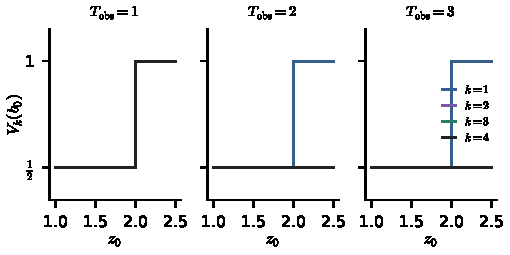
\includegraphics[width=\linewidth]{figs_bs2/fig_staircase.pdf}
\caption{The closed-form values of Corollary \ref{cor:closed} on the
delayed grid: flat at \(\tfrac{1}{2}\) while a branch falls, jumping by
exactly \(\tfrac{1}{2}\) at \(z_{0} = 1 + \min(k, T_{\mathrm{obs}})\),
constant beyond.}
\label{fig:staircase}
\end{figure}

\subsection{The deterministic limit and the two operators}\label{deterministic}

\begin{remark}[the two operators]\label{rem:operators}
The expectation over the disturbance law and the adversarial reading of
its support are \emph{different Bellman operators}. Proposition
\ref{prop:degen} states the deterministic degeneration as a change of
operator: when the kernels are deterministic the stochastic expectation
is replaced by the robust (adversarial-support) reading, and the
resulting value is the robust value of the companion papers. The
degeneration is a theorem about the robust operator; it is not a claim
about the stochastic plant, whose expectation and robust readings differ
in general (Section \ref{scope}).
\end{remark}

\begin{proposition}[survived-mass formula]\label{prop:degen}
Let the kernels be deterministic, \(x^{+} = F(x, a, d)\), and let the
disturbance be read adversarially within its support --- the robust
operator of Remark \ref{rem:operators}. Let the window be blind with
declared sequential class \(\Pi_{B}\). Then the degenerated value is the
\emph{survived-mass formula}
\[
V_{k}(b) = \max_{(u_{0},\dots) \in \Pi_{B}}\;
\sum_{x \in \mathrm{supp}\, b} b(x)\,
\mathbf{1}\bigl[ x \text{ survives } (u_{0}, \dots) \bigr],
\]
a maximum of rational linear functions of \(b\) (the surviving indicators
are the degenerate alpha-vectors). Consequently: if the support \(B\)
carries a jointly surviving blind sequence, \(V_{k}(b) = 1\); and if every
declared sequence loses some branch, then
\(V_{k}(b) \le 1 - \min_{x \in B} b(x)\) --- the robust common-action
verdicts and the minimal-mass deficit bound of the companion papers,
recovered as exact values of the robust operator.
\end{proposition}

With deterministic kernels the posterior support follows the set-valued
recursion, survival from a branch under a fixed sequence is a
deterministic event, and prior mass sums over surviving branches;
maximizing over declared sequences gives the formula, from which both
consequences are immediate (a lost branch carries at least the minimal
mass).

On the two-floor chance instance --- states \(\{0, 1\}\), actions
\(u \in \{\tfrac{2}{5}, \tfrac{3}{5}\}\), state \(0\) surviving exactly
the lower action and state \(1\) exactly the higher --- the one-step
servable sets are \(\Gamma_{1} = \{(1,0), (0,1)\}\) and
\(V_{k}(b_{0}) = \tfrac{1}{2}\) for all audited \(k \le 5\): the chance
deficit \(\delta = \tfrac{1}{2}\) is attained, and the deficit equals the
minimal mass (Figure \ref{fig:twofloor}).

The asymmetric audit prices the deficit beyond the symmetric case. At
\((z_{0}, T_{\mathrm{obs}}) = (\tfrac{3}{2}, 2)\) with prior masses
\(w = \tfrac{3}{10}\) and \(\tfrac{7}{10}\), the four blind two-step
sequences survive
\(\{ \tfrac{3}{10}, \tfrac{3}{10}, \tfrac{7}{10}, \tfrac{7}{10} \}\)
(Table \ref{tab:masses}): every sequence loses a branch, so
\(V_{2}(b_{0}) = \tfrac{7}{10}\) and the deficit \(\tfrac{3}{10}\) equals
the minimal mass --- the degenerate bound of Proposition
\ref{prop:deficit} attained off the symmetric prior (Figure
\ref{fig:masses}).

\begin{table}[t]
\centering
\footnotesize
\caption{The asymmetric audit at
\((z_{0}, T_{\mathrm{obs}}) = (\tfrac{3}{2}, 2)\),
\(b_{0} = (\tfrac{3}{10}, \tfrac{7}{10})\): survived mass of each blind
two-step sequence. Every sequence loses a branch; the value is
\(\tfrac{7}{10}\) and the deficit \(\tfrac{3}{10}\) equals the minimal
mass.}
\label{tab:masses}
\begin{tabular}{@{}l c l@{}}
\toprule
Sequence & Survived mass & Lost branch\\
\midrule
\((+1, +1)\) & $\tfrac{3}{10}$ & falling branch at step 1\\
\((+1, -1)\) & $\tfrac{3}{10}$ & falling branch at step 1\\
\((-1, +1)\) & $\tfrac{7}{10}$ & falling branch at step 2\\
\((-1, -1)\) & $\tfrac{7}{10}$ & falling branch at step 2\\
\bottomrule
\end{tabular}
\end{table}

\begin{figure}[t]
\centering
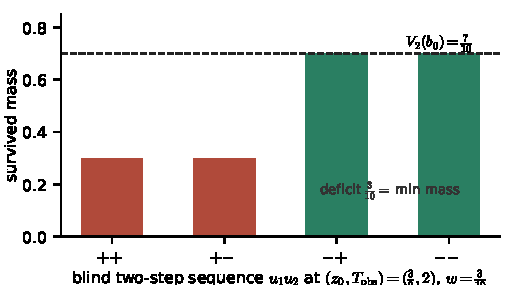
\includegraphics[width=\linewidth]{figs_bs2/fig_masses.pdf}
\caption{The asymmetric audit: survived mass by blind two-step sequence
at \((\tfrac{3}{2}, 2)\) with \(w = \tfrac{3}{10}\). The best sequences
save the heavy branch only; the deficit \(\tfrac{3}{10}\) is the minimal
mass, attained.}
\label{fig:masses}
\end{figure}

\subsection{Certificates as deficit bounds}\label{deficit}

The obstruction certificates bound the deficit from below; their attaining
witnesses are the deficit's dual objects --- computed lower-bound sides of
the exact value, not surrogates for it.

\begin{proposition}[deficit lower bounds]\label{prop:deficit}
Write \(\Delta_{k}(b) = 1 - V_{k}(b)\) for the deficit, and let \(W_{k}\)
denote the \(k\)-step robust kernel in belief space: the family of beliefs
whose support admits a jointly surviving declared-class sequence. Each
companion certificate is a computable lower bound on the deficit.
(i) \emph{Chance-constrained common action:} if the one-step violation
probabilities satisfy \(\sum_{x} b(x)\, p(x, a) \ge \delta\) for every
\(a \in A\), then \(\Delta_{k}(b) \ge \delta\) for every \(k \ge 1\).
(ii) \emph{Degenerate minimal mass:} at the deterministic limit, if
\(b \notin W_{k}\) (the support admits no jointly surviving declared
sequence), then \(\Delta_{k}(b) \ge \min_{x \in \mathrm{supp}\, b} b(x)\)
--- the two-floor instance attains \(\delta = \tfrac{1}{2}\), and on the
delayed grid at \((z_{0}, T_{\mathrm{obs}}) = (\tfrac{3}{2}, 2)\) every
blind sequence loses a branch, so the deficit is at least the minimal
mass \(\tfrac{3}{10}\) of the audited asymmetric prior, attained
(Table \ref{tab:masses}).
(iii) \emph{Monotone deficit:} \(V_{k+1}(b) \le V_{k}(b)\), so the
deficit is non-decreasing in the horizon; on the certified nonviability
region of the delayed grid the deficit is constant.
For finite horizons the exact deficit
\(1 - \max_{\alpha \in \Gamma_{k}} \alpha^{\top} b\) is computable, and
the bounds are witnesses of it, not surrogates.
\end{proposition}

\subsection{Agreement on the delayed-regime class}\label{agreement}

The delayed hidden-regime instance of the calculus paper --- regimes
\(\theta \in \{-1, +1\}\), blind window \(T_{\mathrm{obs}}\), declared
hold class \(\{u \equiv \pm 1\}\), prior \((\tfrac12, \tfrac12)\) from
\(z_{0}\) --- is the agreement test bed. The class declaration is part of
the model: the blind-window policy may be required to hold one action
throughout the window (the declared hold class), or may act sequentially
without observation, or may act with open-loop time-variation.

\begin{theorem}[certificate--value agreement]\label{thm:agree}
On the audited grid (\(z_{0} \in \{1.0, \dots, 2.5\}\),
\(T_{\mathrm{obs}} \in \{1,2,3\}\); 48 cells), over the declared hold
class, and horizons \(k \le 4\):
(a) the class-restricted alpha-vector recursion of Proposition
\ref{prop:pl} returns exactly the closed form of Corollary
\ref{cor:closed} (on the audited grid the second indicator of the
\(k \le T_{\mathrm{obs}}\) line is vacuous, \(z_{0} + k \ge 2\); it is
retained for branch symmetry);
(b) the certificate partition coincides with the value boundaries:
``viable'' iff \(V_{k} \equiv 1\); common-action-certified iff
\(V_{1}(b_{0}) < 1\); timing-certified iff \(V_{1}(b_{0}) = 1\) but
\(V_{T_{\mathrm{obs}}+1}(b_{0}) < 1\);
(c) the attaining witness family changes exactly at \(z_{0} = 2\) at the
one-step horizon and at \(z_{0} = 1 + k\) at horizon
\(k \le T_{\mathrm{obs}}\) (in particular at \(z_{0} = 3\), not \(2\),
for \(k = 2\) with \(T_{\mathrm{obs}} \ge 2\)), and read as a function of
the continuous parameter \(z_{0}\) the hold-class value has jump
discontinuities exactly at \(z_{0} = 1 + \min(k, T_{\mathrm{obs}})\) --- a
jump of exactly \(\tfrac{1}{2}\), from \(\tfrac{1}{2}\) to \(1\) --- these
loci being the certificate edges on the grid (kinks in the strict sense
belong to the piecewise-linear value as a function of the belief, not of
\(z_{0}\));
(d) the deficit equals \(\tfrac{1}{2}\) on every nonviable cell of the
symmetric prior --- the minimal-mass bound attained with the minimal
prior.
\end{theorem}

\begin{proof}[Derivation of the jump loci]
Fix \(T_{\mathrm{obs}}\) and \(k\). On the closed form: if
\(k \le T_{\mathrm{obs}}\) the value is
\(\tfrac{1}{2}(\mathbb{1}[z_{0} \ge 1 + k] + 1)\), the second indicator
being identically one on the grid; it jumps by exactly \(\tfrac{1}{2}\)
at \(z_{0} = 1 + k\). If \(k > T_{\mathrm{obs}}\) the value is
\(\tfrac{1}{2}(1 + \mathbb{1}[z_{0} \ge 1 + T_{\mathrm{obs}}])\),
jumping by exactly \(\tfrac{1}{2}\) at \(z_{0} = 1 + T_{\mathrm{obs}}\).
Both loci are \(z_{0} = 1 + \min(k, T_{\mathrm{obs}})\); between jumps
both expressions are constant in \(z_{0}\). The witness family changes
exactly at the same loci: the attaining one-step vector is \((1, 1)\) on
\(z_{0} \ge 2\) and \((1, 0)\) below, and at horizon \(k\) the change
sits at \(z_{0} = 1 + \min(k, T_{\mathrm{obs}})\).
\end{proof}

\begin{theorem}[class declaration]\label{thm:class}
The declared hold class and the unrestricted sequential blind class
coincide at the one-step horizon. For horizons \(k \ge 2\) they differ
exactly on the timing cells --- those with
\(2 \le z_{0} < 1 + T_{\mathrm{obs}}\) --- and there open-loop
time-variation within the blind window lifts the value to one: an
alternating hold sequence keeps both branches at or above the floor
whenever \(z_{0} \ge 2\), which no constant hold does. On the
common-action cells \(z_{0} < 2\) the restriction costs nothing --- no
blind sequence saves both branches --- and on the viable cells both
classes attain one. On the audited grid the difference comprises exactly
the 12 timing cells at each of \(k = 2, 3, 4\): 36 cell-horizon
combinations in all (Figure \ref{fig:classdiff}).
\end{theorem}

\begin{proof}[Derivation of Theorem \ref{thm:class}]
At \(k = 1\) both classes choose one blind action, so they coincide. Let
\(k \ge 2\) and write the two branch positions after a blind sequence
\(u_{1:\ell}\), \(\ell = \min(k, T_{\mathrm{obs}})\), as
\(z_{0} \pm \sum_{t} u_{t}\). If \(z_{0} < 2\), some branch sits below
\(2 - (z_{0} - 1)\) steps from its floor, and since the partial sums of
any \(\pm1\)-sequence move one branch down whenever they move the other
up, one branch reaches its floor: no blind sequence saves both, both
classes give \(\tfrac{1}{2}\), no difference. If
\(z_{0} \ge 1 + T_{\mathrm{obs}}\) the constant hold already survives
the window on both branches and both classes attain one. On the timing
cells \(2 \le z_{0} < 1 + T_{\mathrm{obs}}\): a constant hold drives the
falling branch to \(z_{0} - \ell < 1\) (deficit), while the alternating
sequence has partial sums in \(\{0, \pm 1\}\), so both branches stay at
or above \(z_{0} - 1 \ge 1\) through the window, and revelation at
\(T_{\mathrm{obs}}\) then regenerates both: the unrestricted class
attains one while the declared class does not. This locates the
difference setwise.
\end{proof}

\begin{remark}[the timing obstruction is class-scoped]\label{rem:scope}
The calculus paper's timing certificates (\(\sigma^{*}(B_{0}) = z_{0} -
1\), \(T_{\mathrm{obs}} < \sigma^{*}\)) are statements about the declared
hold-until-review class --- the institutional reading of a sampled-review
regulator. Theorem \ref{thm:class} quantifies the contrast: within the
declared class the timing cells are nonviable with deficit exactly
\(\tfrac{1}{2}\); under the unrestricted sequential blind class the same
cells attain value \(1\) by oscillation, and no other cell differs. The
timing obstruction therefore certifies exactly what it claims ---
nonviability \emph{within the declared class} --- and no statement of the
companion papers is altered by this reading. The word ``adaptive'' is
avoided for blind windows: while the window is blind, no observation
updates the belief, and the only distinction available is hold-constant
versus time-varying open-loop control.
\end{remark}

\begin{figure}[t]
\centering
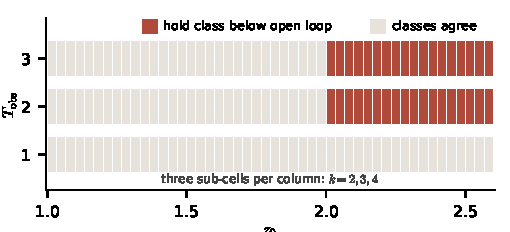
\includegraphics[width=\linewidth]{figs_bs2/fig_classdiff.pdf}
\caption{The class declaration on the audited grid: red cells mark
cell-horizon combinations where the declared hold class and the
unrestricted open-loop class differ --- exactly the timing cells
(\(2 \le z_{0} < 1 + T_{\mathrm{obs}}\)) at horizons \(k = 2, 3, 4\)
(three sub-cells per column); 36 combinations in all. The classes agree
at \(k = 1\), on the common-action cells, and on the viable cells.}
\label{fig:classdiff}
\end{figure}

\subsection{Adaptive observation and hidden parameters}\label{adaptive}

Observation is a design variable. Structural uncertainty --- a hidden
parameter resolved too late, rather than noisy data --- is the
obstruction: the state augments with a hidden parameter
\(\theta \in \Theta\), the belief lives on the product
\((x, \theta)\), and the obstruction is the emptiness of the joint
floor-servable set over \((x, \theta)\) cells. On the declining instance
the parameter \(\theta \in \{-1, +1\}\) gates the correctable component
of a \(-\tfrac{1}{10}\) drift; the list of affected sustainability
parameters --- regeneration rates, climate sensitivity, institutional
effectiveness --- motivates the model class, and the paper verifies on
exact instances.

\begin{proposition}[probes and learning deadlines]\label{prop:learn}
On the audited grid, with quantized control \(u \in \{-1, 0, 1\}\) and
hold-then-probe-then-act schedules: with \(\theta\) observed, every cell
is viable (16 of 16). Under one-probe endogenous learning, the probe
reveals \(\theta\) exactly --- the branch separation is \(2\), so one
observation splits the belief with no statistics --- but survival forces
\(z_{0} \ge 21/10\). Under exogenous revelation at horizon
\(T_{\mathrm{learn}}\), viability holds exactly when
\[
z_{0} \;\ge\; \frac{21}{10} \;+\; \frac{T_{\mathrm{learn}}}{10},
\qquad T_{\mathrm{learn}} = 0, 1, 2, 3, 4,
\]
the learning-deadline identity: late resolution acts as the timing
obstruction's observation deadline, and the kernel shrinks exactly
linearly and antitone in it, \(|K| = 5, 4, 3, 2, 1\) on the grid for
\(T_{\mathrm{learn}} = 0, 1, 2, 3, 4\) (Table \ref{tab:deadline} and
Figure \ref{fig:deadline}). A two-patch instance with unknown
regeneration rate \(g \in \{1, 2\}\) shows the same phenomenon on the
audited two-patch belief pair: unknown-regeneration nonviable,
\((x, g)\)-observed viable.
\end{proposition}

\begin{proof}
Before \(T_{\mathrm{learn}}\) the drift is \(-\tfrac{1}{10}\) (hold
\(u=0\)), so survival to the probe forces
\(z_{0}-\tfrac{T_{\mathrm{learn}}}{10}\ge\) the probe threshold; the
probe \(u=+1\) moves \(z\) by \(-\tfrac{1}{10}+\theta\), which must stay
safe on both branches, giving the threshold \(\tfrac{21}{10}\) at
\(T_{\mathrm{learn}}=0\); after the probe the learned law \(u=\theta\)
has drift \(-\tfrac{1}{10}+\theta^2=\tfrac{9}{10}>0\), so survival is
indefinite. The branch positions
\(z_{0}-\tfrac{1}{10}T_{\mathrm{learn}}-\tfrac{1}{10}\pm1\) differ by
\(2\), so the post-probe reading determines \(\theta\) uniquely.
Antitonicity is the threshold identity; strictness on the grid is the
computed counts \(5,4,3,2,1\).
\end{proof}

\begin{table}[t]
\centering
\footnotesize
\caption{The learning-deadline audit: the exact threshold
\(\tfrac{21}{10} + \tfrac{T_{\mathrm{learn}}}{10}\) and the resulting
kernel on the grid at each deadline.}
\label{tab:deadline}
\begin{tabular}{@{}l c c l@{}}
\toprule
\(T_{\mathrm{learn}}\) & Threshold & \(|K|\) & Kernel \(K\) on the grid\\
\midrule
0 & $21/10$ & 5 & $\{2.1, 2.2, 2.3, 2.4, 2.5\}$\\
1 & $22/10$ & 4 & $\{2.2, 2.3, 2.4, 2.5\}$\\
2 & $23/10$ & 3 & $\{2.3, 2.4, 2.5\}$\\
3 & $24/10$ & 2 & $\{2.4, 2.5\}$\\
4 & $25/10$ & 1 & $\{2.5\}$\\
\bottomrule
\end{tabular}
\end{table}

\begin{figure}[t]
\centering
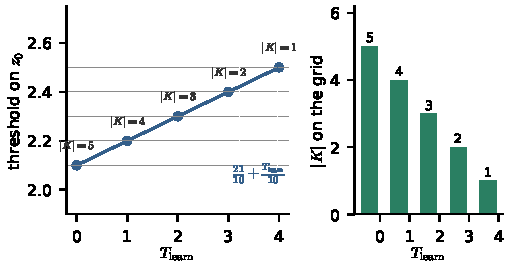
\includegraphics[width=\linewidth]{figs_bs2/fig_deadline.pdf}
\caption{The learning-deadline identity: the viability threshold
increases exactly linearly in \(T_{\mathrm{learn}}\) (left), and the
kernel on the grid shrinks linearly and antitone, \(|K| = 5, 4, 3, 2,
1\) (right).}
\label{fig:deadline}
\end{figure}

\begin{figure}[t]
\centering
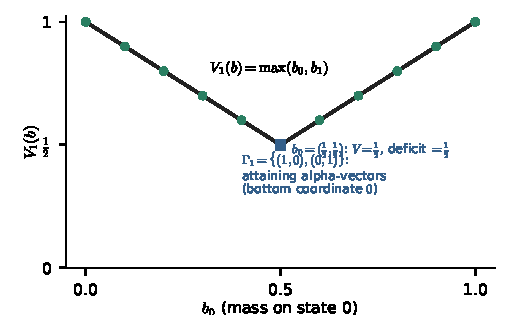
\includegraphics[width=0.88\linewidth]{figs_bs2/fig_twofloor.pdf}
\caption{The two-floor chance instance: the one-step value is
\(\max(b_{0}, b_{1})\), attained by the alpha-vectors of
\(\Gamma_{1} = \{(1,0), (0,1)\}\) with zero bottom coordinate (green
probes); at the symmetric prior the value is \(\tfrac{1}{2}\) and the
deficit equals the minimal mass.}
\label{fig:twofloor}
\end{figure}

\subsection{Verification methods}\label{methods}

Every value, bound, identity, threshold, figure, and tabulated entry in
this paper is regenerated by deterministic scripts in exact integer and
rational arithmetic, standard library only. Three per-system scripts
cover the audited instances, and one master entry point chains them.
The belief-state campaign script runs sixteen check families on the
stochastic values (the two-floor instance, piecewise-linearity, the
deterministic limit, the 48-cell agreement, the partition coincidence,
the witness family, the deficit identity, the unrestricted class,
rationality of all 384 campaign alpha-vectors, deficit monotonicity, the
oscillation identity, model completeness, the selector split, dimension
consistency, the jump loci, and the declarations), chaining two
per-instance scripts of twenty-one further checks. The stochastic
selector script re-derives every selector claim in fifteen check
families (S1--S15: the two-floor backup, eleven-belief piecewise
linearity, degeneration against brute force, 48-cell closed-form
agreement, partition coincidence, witness-family loci, the exact
deficit on all 42 nonviable cells, the class declaration by brute
force, rationality of the 384 vectors, monotonicity, the oscillation
identity to horizon 24, model completeness, the selector split,
dimension padding, and the one-sided jump values). The hidden-parameter
script runs six check families on the adaptive-observation instance
(theta observed on all 16 cells, the probe threshold
\(\tfrac{21}{10}\) as a branchwise identity, the deadline identity at
\(T_{\mathrm{learn}} = 0, \dots, 4\), injective revelation, the
antitone kernel chain, and the unknown-regeneration two-patch
instance). The master script for this paper chains the three, then
recomputes independently from the definitions: the closed-form values on
the whole \(16 \times 12\) grid by direct branch-mass enumeration, the
resulting census (\(36\) unit values and \(156\) half values on the
declared class), the identity of the class-difference set with the
timing-cell combinations at \(k \ge 2\) by brute-force enumeration over
blind sequences, the \(384\)-vector type census (\(156\), \(156\),
\(72\)), the deficit \(\tfrac{3}{10}\) of the asymmetric audit sequence
by sequence, the learning-deadline threshold chain
\(\tfrac{21}{10} + \tfrac{T_{\mathrm{learn}}}{10}\), and every headline
number asserted present in the text and bound to the chained scripts'
certified families.

\subsection{Delimitations and outlook}\label{scope}

The semantics here is stochastic expectation: the value is a survival
\emph{probability}, and the robust quantifiers of the companion papers
are recovered only at the deterministic degeneration, which is a change
of operator (Remark \ref{rem:operators}); the stochastic and robust
readings of a genuinely stochastic plant differ, and this paper does not
conflate them. The timing layer's statements, here and in the companion
papers, are class-scoped (Remark \ref{rem:scope}). No learning theory is
claimed beyond the one-probe exact split: Bayesian updating, repeated
experiments, and exploration--exploitation trade-offs are out of scope;
the deadline result is for the audited schedule family (hold, probe,
learned act), and other schedules are not classified; the parameter
\(\theta\) enters additively, and state-dependent parameter dynamics
belong to the hybrid companion's setting. The alpha-set growth is
exponential in the worst case; the agreement theorem's classes are
two-witness instances precisely because the audited systems are. General
information structures beyond history partitions (control-dependent
observations, active sensing), continuous-time exit-time value functions,
and second-moment (conic) relaxations of the support-function rows are
the next items of the programme; the deficit-bound reading of
Proposition \ref{prop:deficit} is the interface through which this
theory attaches to the certificate families already established, and the
exact rational values of the audited campaign are the benchmark any
such relaxation must meet.

\subsection{Conclusion}\label{conclusion}

The belief-state safety value carries the obstruction calculus into the
probabilistic setting without loss of exactness. The support identity
ties the value-one level to the viable-set recursion; rational
alpha-vectors keep every audited value exact, and the complete value
table shows the two-valued structure the certificates predict; the
certificates survive as deficit lower bounds, attained on natural
instances on both the symmetric and the asymmetric prior; the audited
delayed-regime class agrees with its closed form cell by cell, with the
class declaration responsible for exactly the 36 timing combinations;
and the adaptive-observation audit prices late resolution exactly --- a
linear learning deadline on the viable set, \(|K| = 5, 4, 3, 2, 1\). The
observation layer, not the forecast layer, sets the value; the design
rules are the same ones the deterministic audits impose, now with a
price attached and every number in the tables open to script-level
re-inspection.

\subsection*{References}

{\footnotesize
Abaee, A. An obstruction calculus for viability under incomplete
observation (submitted).

Abaee, A., 2026a. Robust viability of the 2J3KL limit reference point
under a surplus-production map: policy scoring, expansion, and when
catch cannot help. Zenodo.
\url{https://doi.org/10.5281/zenodo.22552060}

Bertsekas, D.P., Shreve, S.E., 1978. Stochastic Optimal Control: The
Discrete-Time Case. Academic Press, New York.

\`{A}str\"{o}m, K.J., 1965. Optimal control of Markov processes with
incomplete state information. J. Math. Anal. Appl. \textbf{10},
174--205.

Smallwood, R.D., Sondik, E.J., 1973. The optimal control of partially
observable Markov processes over a finite horizon. Oper. Res.
\textbf{21}(5), 1071--1088.
}

\subsection*{Declarations}

\subsection*{Funding}
None.

\subsection*{Competing interests}
None.

\subsection*{Data availability}
No external data were used.

\subsection*{Code availability}
The verification script
\url{paper2_probabilistic_sufficiency_v1_verification.py} --- which chains
the per-system scripts \url{paper2_belief_state_v2_verification.py},
\url{paper2_stochastic_selector_v2_verify.py}, and
\url{hidden_parameter_learning_v1_verify.py} --- and the figure-and-table
generation script \url{paper2_belief_state_figures.py} are publicly
available at \url{https://github.com/MIKEAA2020/general-sustainability}
(folder \texttt{arena agent 1/paper rewrites/latex}, at the commit
pinned to this article's submission); they reproduce all values, bounds,
thresholds, figures, and tabulated entries verbatim.

\subsection*{AI declaration}
GLM (Z.ai), Qwen (Alibaba Cloud) and DeepSeek AI assisted with drafting
and iterative review. The author reviewed and edited outputs and takes
responsibility for the final work.

\end{document}
